\documentclass[10pt,a4paper]{article}
\usepackage[utf8]{inputenc}
\usepackage{amsmath}
\usepackage{amsfonts}
\usepackage{amssymb}
\usepackage{tcolorbox}
\usepackage{graphicx}
\usepackage[numbers]{natbib}
\usepackage[margin=0.8in]{geometry}
\usepackage{ amssymb }
\usepackage{placeins}
\usepackage{array}

\makeatletter
\newcommand{\thickhline}{%
    \noalign {\ifnum 0=`}\fi \hrule height 1pt
    \futurelet \reserved@a \@xhline
}
\title{Machine Learning Project: Report 2}
\author{Ignace Bleukx \and Quinten Bruynseraede}
\begin{document}
\maketitle
\section{Introduction}
\subsection{Evaluation metrics}
Evaluation of agents is traditionally done using \textbf{NashConv} and \textbf{exploitability}. We introduce these concepts here, using terminology consistent with \citeauthor{lanctot2019openspiel} \citep{lanctot2019openspiel}.

Given a two-player policy$\pi$, we say that $\pi^{b}_{i}$ is the best response for player $i$. The best response is defined as the policy that maximizes payoff for player $i$, given the policies of other players ($pi_{-i}$). 

We then define the incentive to change policies $d_{i}(\pi)$ as $d_{i}(\pi) = u_{i}(\pi^{b}_{i},\pi_{-i}) - u_{i}(\pi)$, i.e. the possible gain in value when switching to a best-response strategy. It is clear that this can be used as a metric to evaluate a policy: a Nash equilibrium is found when $d_{i}(\pi)$ = 0 (the policy cannot be improved given other player's policies). Any value $>0$ captures room for improvement for a given theory. 

From this initial notion of policy evaluation, the \textbf{NashConv} metric is derived as the sum of $d_{i}(\pi)$ for both players.

Another metric that is often used, is \textbf{exploitability}. For two-player zero-sum games (such as the games we will be learning in this assignment), exploitability equals $\frac{NashConv}{2}$. We therefore only use Exploitability to evaluate our policies (as NashConv can be derived from Exploitability in this case).

Looking for Nash equilibria is interesting in zero-sum games because they guarantee a maximal payoff against any policy the other players might have. We will therefore focus on finding approximations of Nash equilibria (i.e. minimizing exploitability). 

\subsection{Normal form - Extensive form}
In game theoretic aspects, two forms of representing a game exists: normal form and extensive form. The normal form description of a game can be represented as a payoff matrix. This means every action for every player must be included in the matrix. This makes the representation extremely incovenient for larger games like leduc poker.
The extstensive form representation of games uses a tree to represent all states of a game. The nodes of this tree represent the descision points in the game for a player. Every branch represents a choice made by a player in the decision point. This representation is much more compact and contains much more information about the course of the game.

\subsection{Algorithm 1: Fictitious Self-Play}
\label{sub:xfsp}
Fictious play is a classic algorithm introduced by \cite{fp}. It's goal is to find the optimal strategy or Nash equilibrium for imperfect games in normal form \cite{MCFSP}. The algorithm is based on the fictitous play of the game, which corresponds to a player simulating a game in it's head and choosing the best response for the current situation. In this simulation, the player assumes the opponent always chooses the best response.

This elegant and simple algorithm has proven to be very successful in relatively small games, however, as stated by \cite{fsp-ext}, the algorithm only works with games in normal form. Extensive-form games can be cconverted into normal form games but the number of actions increases exponentially in the number of game sates \cite{fsp-ext}.
Therefore the Extensive Fictious Play algorithm was developped by \cite{fsp-ext} to support self play for extensive form games.

The algorithm consisists of two steps: finding the best response for the current state, and updating the current average strategy of the agent.
To find the best reponse for the curren state, the game state tree is traversed and the set of best responses is calculated based on the final outcome. Out of this set, a best reponse is selected.
The seconds step is to update the average policy by using the calculated best response. The update rule for the policy is the following:
\begin{math}
\pi_{i+1}(u) = \pi_{i}(u) + \frac{\alpha_{i+1}x_{\beta_{i+1}}(\sigma_{u})(\beta_{i+1}(u) - \pi_i(u))}{(1-\alpha_{i+1})x_{\pi_i}(\sigma_{u}) + \alpha_{i+1}x_{\beta_{i+1}}(\sigma_u)}
\end{math}.\\
Where $\pi_n(u)$ indicates the action probabilities of the policy at iteration $n$, $\beta_n$ the best reponse calcuated in step 1 and $\sigma{u}$ a sequence of actions to reach state $u$. $x{\beta}(\sigma_u)$ is the realization plan for this sequence, given best response $\beta$.\\
The main issue with this form of fictitous play is the computational effort needed to calculate the best response. 
Reinforcement learning can address this problem by using machine learning techniques to approximate the optimal response.
The reinforcement techniques plug in in a framework called FSP or Fictious Self Play. Here, both calculation of the best response and the update of the policy can be substitued by reinforcement learning methods.

\subsubsection{Extension: Neural Fictitious Self-Play}
\label{sub:nfsp}
In the NFSP algorithm, the best response and update rule are approximated by training two neural networks.
\paragraph{Best response}
To calculate the best response, we train a Deep Q-network or DQN. This agent learns an $\epsilon$-greedy policy \cite{heinrichphd}. 
This can be done as the games considered have perfect recall and the history of the game is thus available to the agents. By using this history the agent gains experience and approximates the best response for a given state.
The implementation of NFSP in Openspiel uses a multilayer perceptron network (MLP).
\paragraph{Average Strategy}
To compute the action probabilities for a given state in the game, NFSP trains another ANN which maps these states to the corresponding probabilities. The network is trained by using information of past actions performed. As the average policy is approximated, the network does not need to be consulted every iteration of the learning process. This means the update can be much more effecient when using a good ANN.
In the Openspiel implementation of NFSP this is an MLP.
\subsection{Algorithm 2: Counterfactual Regret Minimization}
\label{sub:cfr}
Counterfactual Regret Minimization (CFR in short) is an algorithm that is designed to find Nash equilibria in large games. It introduces the notion of counterfactual regret, and minimizes this to compute a Nash Equilibrium. \citeauthor{cfr} \citep{cfr} show that CFR can solve games with up to $10^{12}$ states, such as Texas Hold'em. We therefore expect it to perform well on reduced variants of traditional poker, such as Kuhn and Leduc poker.\\

An important concept in reinforcement learning is the notion of regret, which can be paraphrased as the difference between maximum and actual payoff an agent receives when executing a sequence of steps. The goal of many reinforcement learning algorithms is to minimize regret. What makes regret minimization less applicable in large games, is that regret is to be minimized over all game states. This quickly becomes infeasible when dealing with a large number of states. The general idea of counterfactual regret minimization is to decompose regret into a set of regret terms, whose som approaches the actual regret. \citeauthor{cfr} then show that individually minimizing these regret terms leads to a Nash equilibrium. We will now introduce counterfactual regret minimization more formally, based on \citep{cfr_for_beginners}\\

\begin{itemize}
\item{A history $h$ is a sequence of actions performed by the agents, starting from the root of the game tree (the initial state). }
\item{An information state $I$ consists of a player and the information that is visible to that player.}
\item{All player have their individual strategies, and we call the combination of these strategies at time $t$: $\sigma^t$. $\sigma^t_{I \rightarrow a}$ denotes a strategy identical to $\sigma$, but action $a$ will always be taken in information state $I$.}
\item{Counterfactual ($-i$) refers to excluding the probabilities of actions that player $i$ took, as if he guided (with action probabilities 1) the game towards a certain history or information. We can use this definition to calculate $P^{\sigma}_{-i}(h)$ and $P^{\sigma}_{-i}(I)$.}
\item{The counterfactual value of a history $h$ under a joint strategy $\sigma$ is defined as:
\begin{equation}
v_{i}(\sigma,h) = \sum_{z \in Z, h \sqsubset z }{P^{\sigma}_{-i}(h)P^{\sigma}(h,z)u_i(z)}
\end{equation}
where $Z$ denotes the set of possible terminal game histories, and $h$ is any non-terminal subhistory of $z \in Z$. This equation captures that the value of a certain history has to be weighed to account for the counterfactual probabilities. More specifically, the actions of other players (where chance influences their play) influence the probability of a history, which is taken into account.}
\item{The counterfactual regret is defined as:
\begin{equation}
r(h,a) = v_{i}(\sigma_{I \rightarrow a},h) - v_{i}(\sigma,h)
\end{equation}
This regret captures how much value was lost by \textit{not} picking action $a$, as opposed to a strategy that does execute $a$ in history $h$.}
\item{The counterfactual regret of not taking an action $a$ in information state $I$ is simply the sum of regret of all histories in $I$:
\begin{equation}
r(I,a) = \sum_{h \in I}{r(h,a)}
\end{equation}}
\item{Finally, the cumulative counterfactual regret of not taking action $a$ in information state $I$ if called $R^T(I,a)$ and can be expressed as the sum of regrets at all time steps:
\begin{equation}
R^T(I,a) = \sum_{t=1}^{T}{r(h,a)}
\end{equation}}
\end{itemize}

As expected, the goal is to locally minimize this regret for each information state. This is done iteratively. In each step, a strategy can be extracted from the counterfactual regrets. One way of doing this is using regret matching, where action probabilities are computed proportional to positive regrets. For example, a high positive regret indicates that small losses have been experienced when not picking a certain an action. It is therefore interesting to perform this action more often, and it will be given a higher weight.

Openspiel uses Hart and Mas-Colell's regret-matching algorithm, which obtains a new strategy $\sigma^{T+1}$ in the following way:
\begin{equation}
\sigma_{i}^{T+1}(I,a) = 
	\begin{cases}
	\frac{R_{i}^{T,+}(I,a)}{\sum_{a \in A(I)}{R_{i}^{T,+}(I,a)}} \text{ if denominator }> 0 \\
	\frac{1}{|A(I)|} \text{ otherwise}\\
	\end{cases}
\end{equation}

In this equation, $A(I)$ denotes the set of actions that can be taken in information state I, and $R^+$ is obtained by bounding regret values in the interval $\mathclose[0,\infty\mathclose[$. The value of $\sigma^{T+1}$ is calculated for each information state and each action to obtain a complete strategy.

It should be noted that the average strategy converges to a Nash equilibrium, and not the final strategy. When discussing results of policies obtained using CFR, it is implicitly assumed we have extracted the average policy after training.

Most succesful approaches to learning large imperfect-information games (such as Kuhn Poker and Leduc Poker) are based on CFR. We will now take a closer look at two variants of classical CFR, that try to overcome the limitations of strictly tabular approach. When the number of states is very large, it becomes increasingly infeasible to calculate counterfactual regret values for each and every information state. To solve this, abstraction is often introduced: aggregating information states to reduce the size of the game. Regression CFR applies the principle of abstraction. Deep CFR uses a deep learning to approximate CFR, without using abstraction.\citep{dcfr}

\subsubsection{Extension: Regression Counterfactual Regret Minimization}
\label{sub:rcfr}
Regression CFR (introduced by \citeauthor{regression_cfr} \citep{regression_cfr}) is an extension of CFR where counterfactual regret values are not stored in a tabular format, but estimated using a function $\phi: I \times A \mapsto \mathbb{R}$., that maps each combination of a (visible) information state and an action to an estimation of the counterfactual regret value.\\

One interesting property of using regression CFR (RCFR) is the fact that a game can be abstracted down using a appropriate regressor. Consider a game like Texas Hold'em Poker, with roughly $10^{160}$ possible sequences. Storing all counterfactual regret values quickly becomes impossible. A solution is to assign regret values to clusters and estimate a representative for each cluster. This might reduce the number of values to a manageable size. In RCFR, this clustering is done implicitly when choosing a regressor: a simple model such as bounded regression trees will learn rough abstractions, whereas a neural netwerk may not add any abstraction at all. Furthermore, RCFR is able to adapt the regressor $\phi$ on the fly, increasing or decreasing abstraction as needed.\\

As such, we note that using RCFR instead of regular CFR should be used as a technique to make learning more tractable, and not to decrease exploitability. Therefore, the goal should be to approximate the exploitability reached by CFR, but with a reduced number of states.

OpenSpiel supports using RCFR with a user-defined regressor. We chose to use a feedforward neural network. We will examine the results of different network sizes in Section 2 and 3.

\section{Kuhn Poker}
\begin{tcolorbox}
\begin{itemize}
\item{Which algorithm is most suitable to develop an agent to play Kuhn Poker, minimizing exploitability?}
\item{Under which circumstances does RCFR approach classical CFR when learning Kuhn Poker?}
\item{Can we exploit properties of Kuhn Poker to optimize parameters?}
\end{itemize}
\end{tcolorbox}

\subsection{NFSP and XFSP}
In the following section we discuss results of the NFSP and XFSP algorithm (as discribed in \ref{sub:nfsp} and \ref{sub:xfsp}). We use the XFSP algorithm as a baseline, because it is the exact interpretation of the Fictious Self Play algorithm. Next, we optimize different parameters of the NFSP algorithm for Kuhn and Leduc poker. Lastly, we compare the computational effort needed to run both algorithms in different settings.

We use the results of \cite{heinrichphd} as a starting point for Leduc Poker and try to replicate that testing methodology for Kuhn Poker.
First we try to find the optimal size of neural network for Kuhn Poker. This is important as the size of the network greatly influences the training time.
\cite{heinrichphd} suggests an ANN with 1 hidden layer of 64 nodes for the Leduc Poker setting. Therefore, we start with one layer in the Kuhn Poker setting and adapt the number of nodes. The influence of the layer size on the exploitability is shown on the left hand side of \ref{fig:layers_kuhn}
On the right hand side of this figure we plot the influence of the number of hidden layers on the exploitability. We run the algorithm for 25 000 iterations to keep the execution time manageable, while still getting representative results.

\begin{center}
\begin{figure}[h]
\label{fig:layers_kuhn}
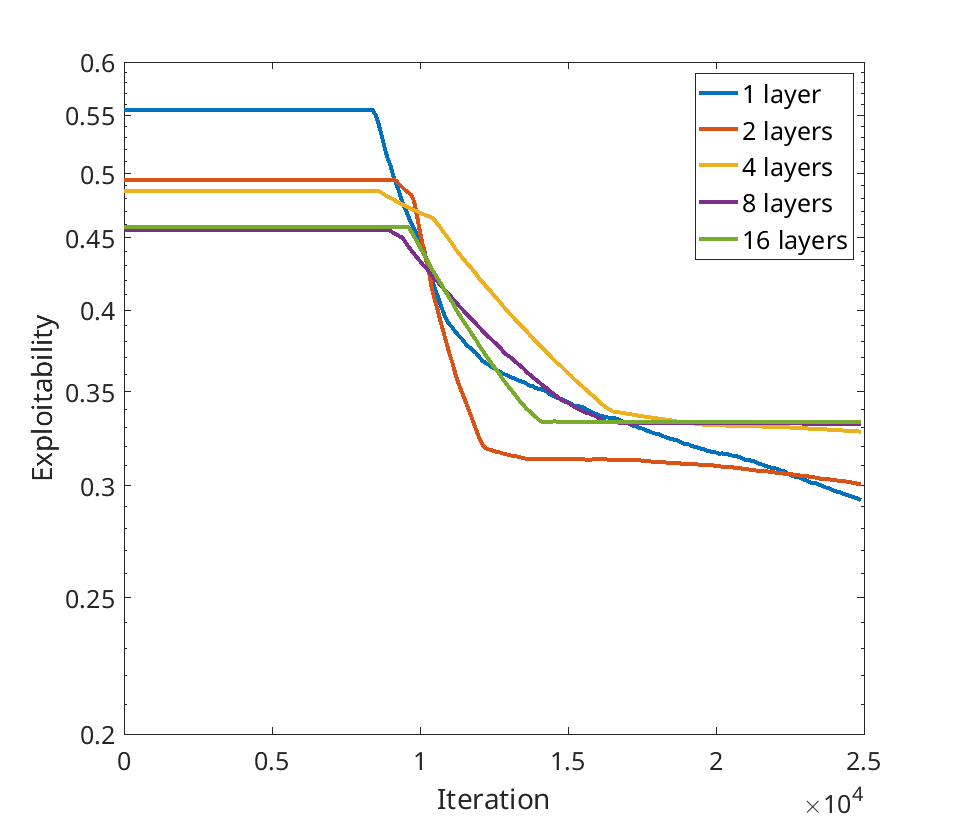
\includegraphics[width=0.5\textwidth]{Figures/kuhn_layers.png}
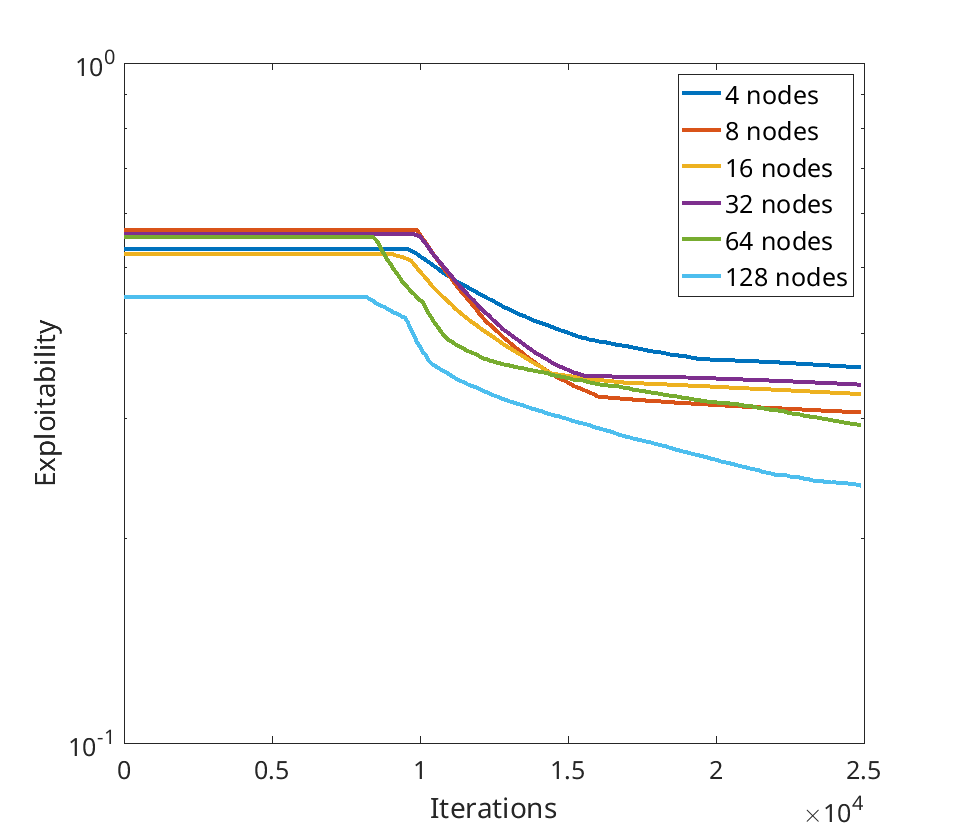
\includegraphics[width=0.5\textwidth]{Figures/kuhn_nodes.png}
\caption{Influence of ANN layer settings in NFSP on exploitability Kuhn Poker}
\end{figure}
\end{center}

We see that the size of layers greatly influences the exploitability when learning Kuhn Poker. As the number of nodes increases, the exploitability drops. However, we find that the sweet spot lies at 64 nodes per layer. This results in a manageable training time and gives good performance.
An important remark is that the algorithm does not improve its exploitability for a long time. Around the 10.000th iteration the exploitability start to drop. 

Assuming that these are good parameters for Kuhn Poker, we compare the optimal settings with the fully fledged XFSP algorithm for the first 60 000 iterations. This number was chosen as the XFSP algorithm does not improve significantly beyond this point. XFSP clearly outperform NFSP in this experiment.

\begin{figure}[h]
\centering
\label{fig:layers_kuhn}
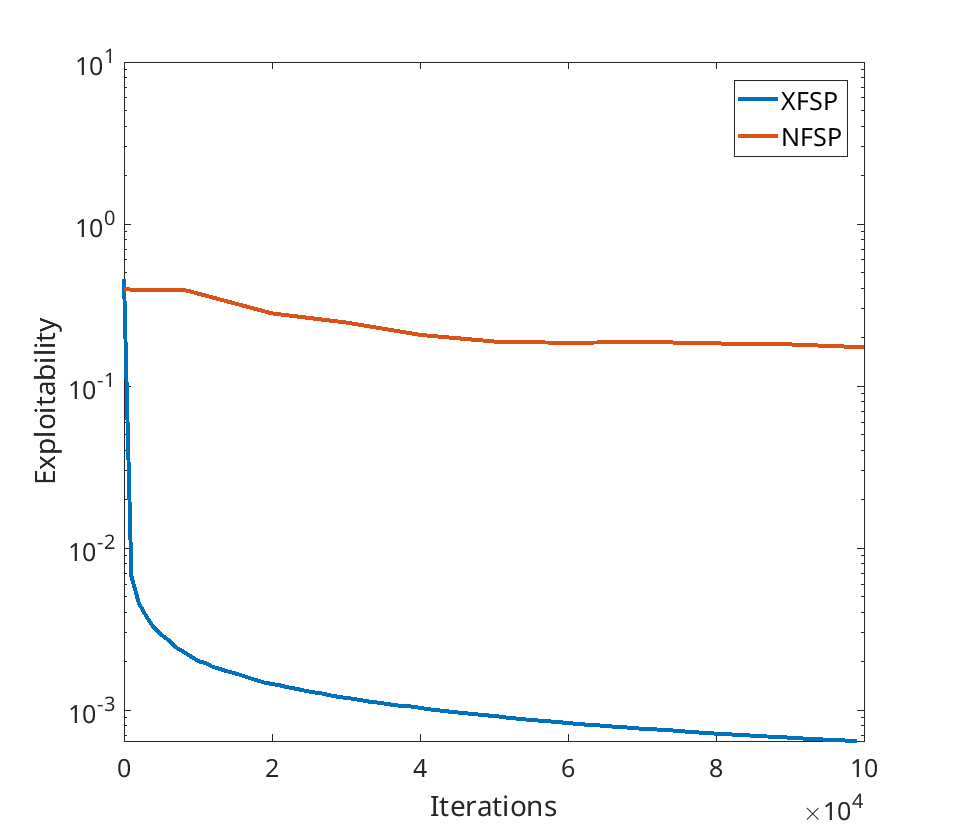
\includegraphics[width=0.5\textwidth]{Figures/xfsp_nfsp_kuhn.png}
\caption{Exploitability of XFSP and NFSP on Kuhn Poker}
\end{figure}

In this last figure, the algorithm NFSP algorithm is ran for 3.000.000 iterations to show what it is capable of. Sadly we were not able to achieve the results for Leduc Poker as described in \cite{heinrichphd}.

% \begin{center}
% \begin{figure}[h]
% \label{fig:full_run_nfsp}
% \centering
% 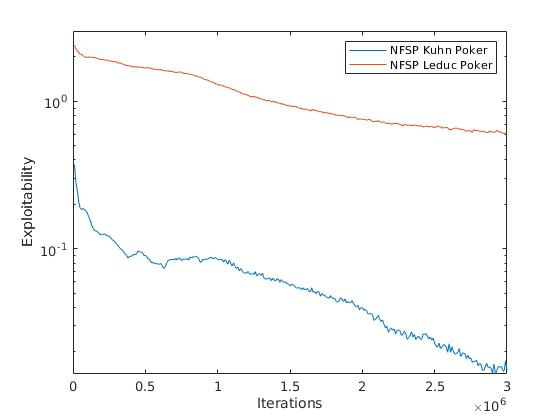
\includegraphics[width=0.5\textwidth]{Figures/nfsp_full_run.jpg}
% \end{figure}
% \end{center}

To conclude this section, we compare the computational effort needed to train the XFSP algorithm and the optimal settings for the NFSP algorithm. From table \ref{tab:time_fsp} we can see the XSFP algorithm is much more computationally intesive then the NFSP algorithm. This makes it unsuitable for larger games. Both Leduc Poker and Kuhn Poker are too small to really show the benefit of using the NFSP algorithm, in our opinion the improved training time of NFSP does not weigh up against the improved exploitability of XFSP.

\begin{tcolorbox}
	Table with times per iteration for NFSP and XFSP
\end{tcolorbox}

\subsection{CFR and RCFR}
In this section, the goal is twofold. First, we analyze how Counterfactual Regret Minimization (CFR, as described in \ref{sub:cfr}) performs when learning Kuhn Poker. Next, we examine under which circumstances RCFR (Regression CFR, see \ref{sub:rcfr}) can be used as a viable alternative to CFR.

As mentioned before, openspiel uses a feedforward neural network as a regressor for RCFR. We can modify the number of layers and hidden nodes per layer. The following graphs show how the number of layers and nodes influences RCFR's performance compared to CFR. We tracked the exploitability of the average policy every 10 iterations. These experiments were limited in length, with only 1000 iterations. Therefore, we will only draw general conclusions, as is it not clear how results generalize to longer experiments. However, based on the graphs and the minimal difference between successive exploitability values, we suspect no large improvements to happen when increasing the number of iterations to 10 000, or 100 000.
 

\FloatBarrier
\begin{figure}[h]
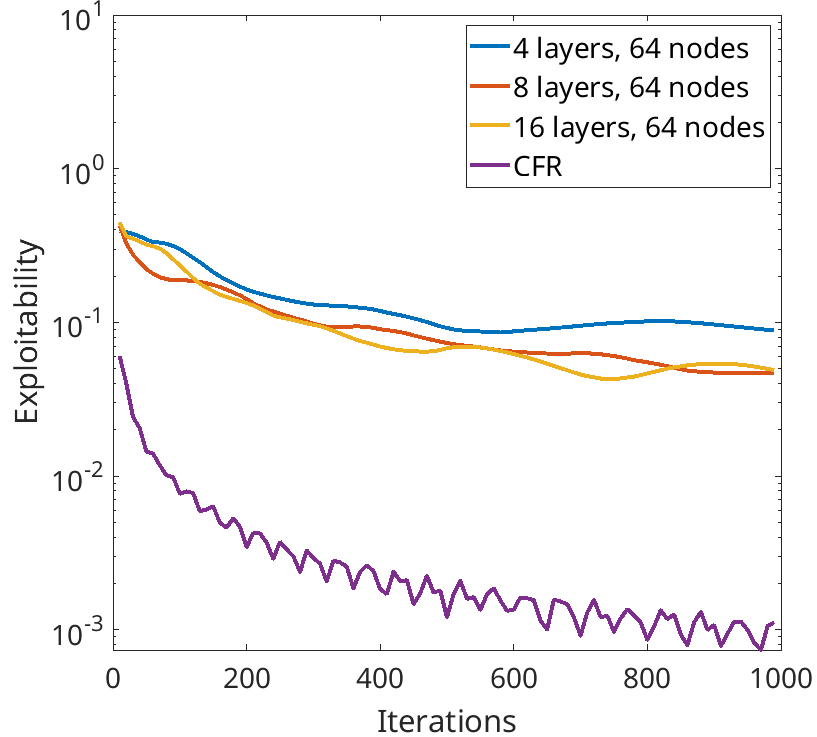
\includegraphics[scale=0.26]{Figures/rcfr_kuhn_parameters1.png}
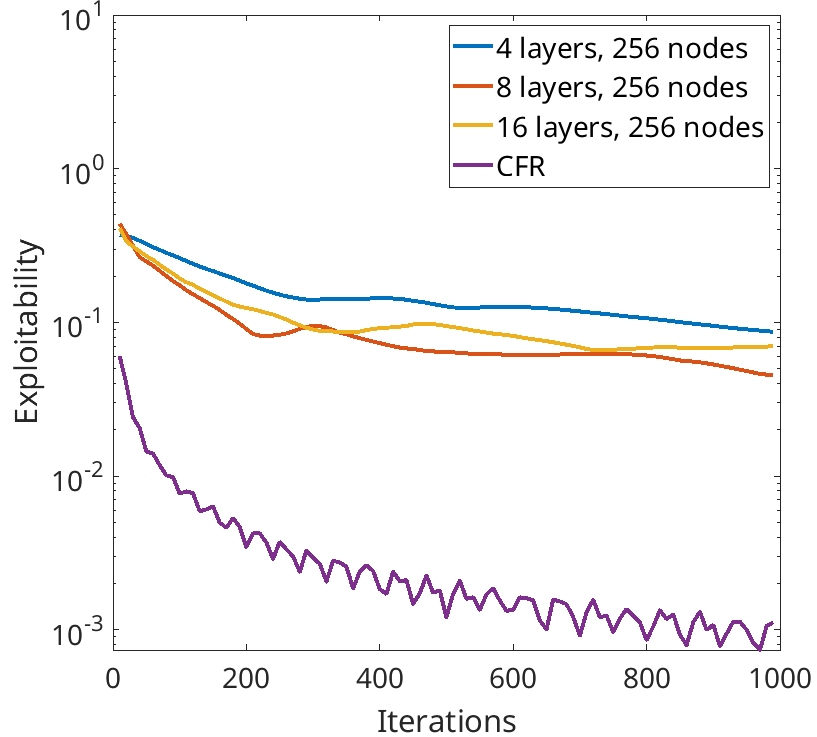
\includegraphics[scale=0.26]{Figures/rcfr_kuhn_parameters2.png}
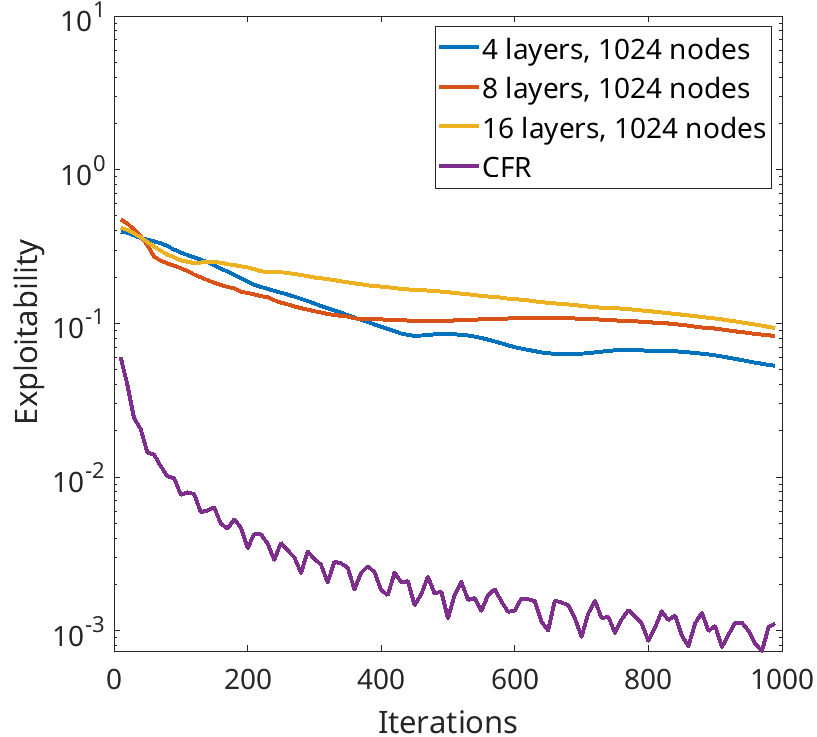
\includegraphics[scale=0.26]{Figures/rcfr_kuhn_parameters3.png}
\caption{Influence of network parameters on CFR and RCFR exploitability}
\label{fig:rcfr_kuhn}
\end{figure}
\FloatBarrier 

It immediately becomes very clear that CFR performs very well when learning Kuhn Poker: the average policy after 1000 iterations has an exploitability of around 1e\textsuperscript{-3}. RCFR struggles to reach these values. The number of layers does not influence the results in a consistent way: it appears that adding more layers and nodes does not make RCFR perform better for Kuhn poker. 

We therefore recommend decreasing the number of layers as much as possible, provided that the exploitability does not appear to worsen. This approach will greatly reduce the time needed to train the agent, as is shown in Table \ref{tbl:kuhn_times}

\begin{table}
\centering
\begin{tabular}{|l|r|}
\hline
Algorithm & Average time per iteration (milliseconds)\\
\thickhline
CFR & 6 \\
\thickhline
RCFR, 4 layers, 64 nodes& 157 \\
\hline
RCFR, 4 layers, 256 nodes & 153 \\
\hline
RCFR, 4 layers, 1024 nodes & 161 \\
\thickhline
RCFR, 8 layers, 64 nodes & 273 \\
\hline
RCFR, 8 layers, 256 nodes  & 270 \\
\hline
RCFR, 8 layers, 1024 nodes  & 235 \\
\thickhline
RCFR, 16 layers, 64 nodes & 486 \\
\hline
RCFR, 16 layers, 256 nodes & 475 \\
\hline
RCFR, 16 layers, 1024 nodes & 498 \\
\hline
\end{tabular}
\caption{Computation time of one iteration for Kuhn Poker, averaged over 50 episodes}
\label{tbl:kuhn_times}
\end{table}

As expected, RCFR is always much slower than CFR. But when using RCFR, increasing and decreasing the number of layers is mainly what impacts the time per iteration. Based on Figure \ref{fig:rcfr_kuhn} and \ref{tbl:kuhn_times}, we conclude that a network of 4 layers and 64 nodes is our current best setting for RCFR. A neural network with these parameters seems to be expressive enough to predict counterfactual regret values. However, 


 


\section{Leduc Poker}
\begin{tcolorbox}
\begin{itemize}
\item{Which algorithm is most suitable to develop an agent to play Leduc Poker, minimizing exploitability?}
\item{Can we exploit properties of Leduc Poker to optimize parameters?}
\item{Under which circumstances does RCFR approach classical CFR when learning Kuhn Poker?}
\end{itemize}
\end{tcolorbox}
\subsection{NFSP and XFSP}
As before, we examine which parameters for the ANN in NFSP give the best results, this time for Leduc Poker. We run the algorithm for 100 000 iterations, as the game is much harder to learn and the results after only 25 000 iterations are not representative.

\begin{center}
\begin{figure}[h]
\label{fig:layers_kuhn}
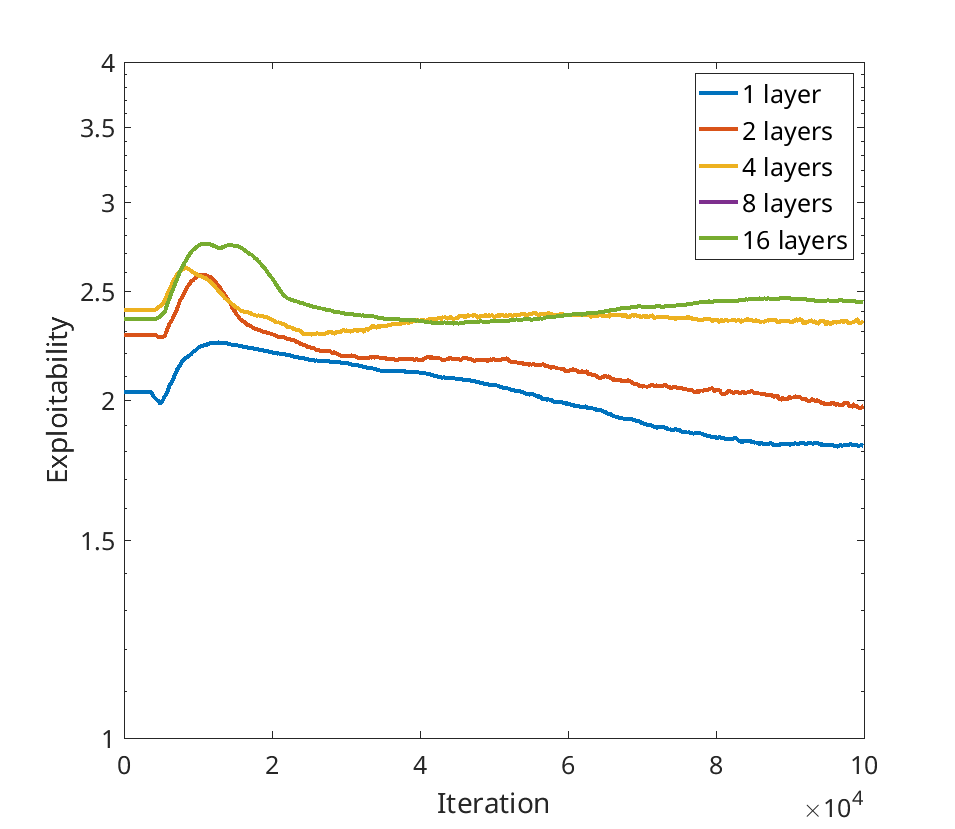
\includegraphics[width=0.5\textwidth]{Figures/leduc_layers.png}
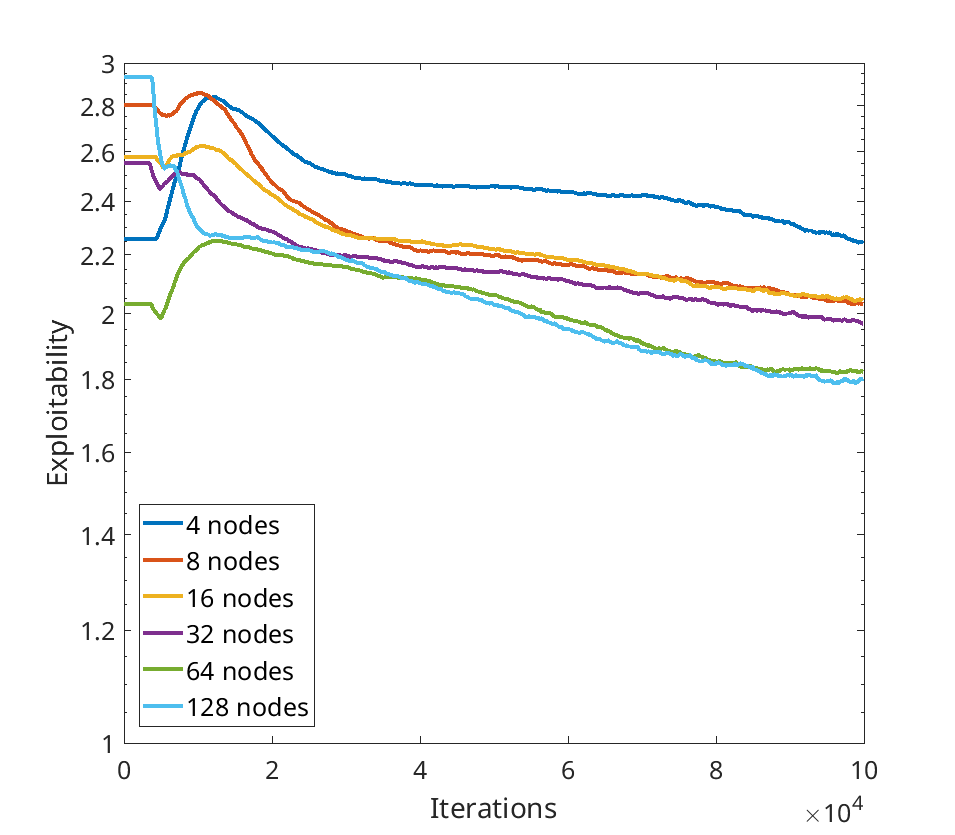
\includegraphics[width=0.5\textwidth]{Figures/leduc_nodes.png}
\caption{Influence of ANN layer settings in NFSP on exploitability Leduc Poker}
\end{figure}
\end{center}


\begin{center}
	\begin{figure}[h]
	\centering
	\label{fig:layers_kuhn}
	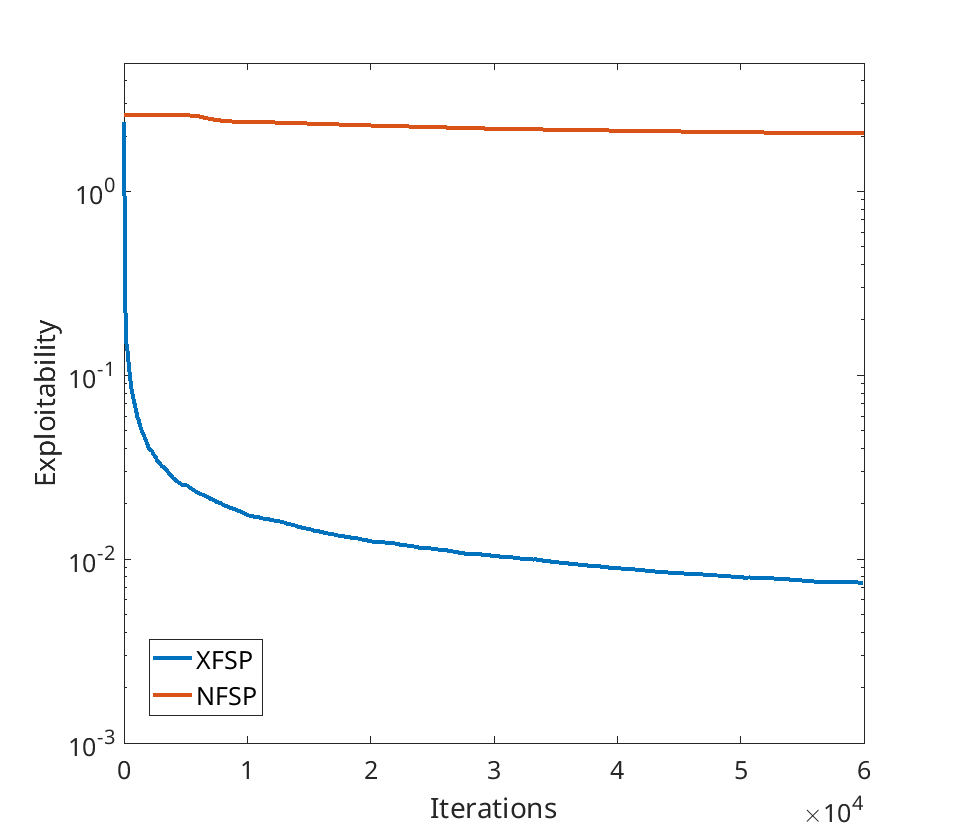
\includegraphics[width=0.5\textwidth]{Figures/xfsp_nfsp_leduc.png}
	\caption{Exploitability when using NFSP and XFSP on Leduc Poker}
	\end{figure}
	\end{center}

\subsection{CFR and RCFR}

\FloatBarrier
\begin{figure}[h]
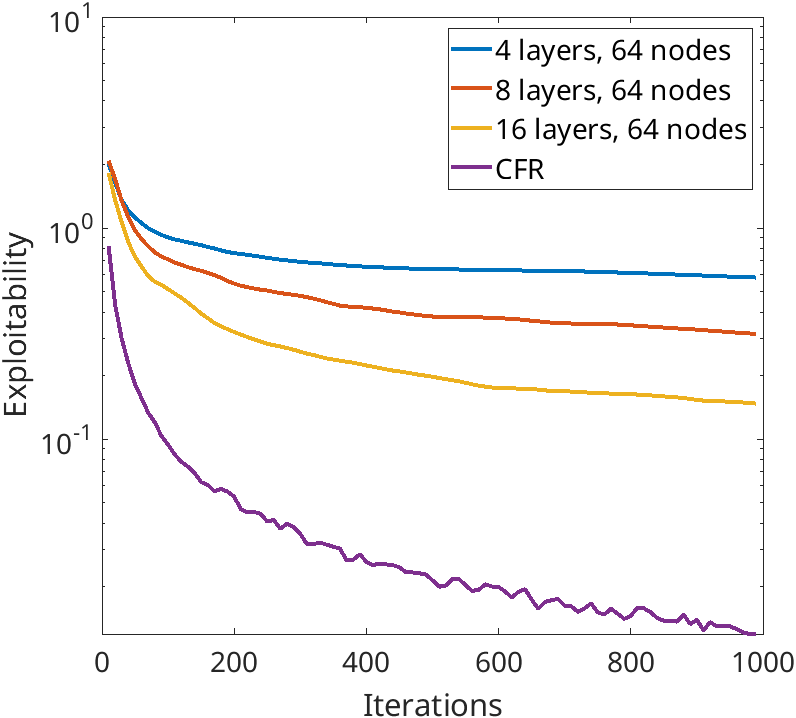
\includegraphics[scale=0.26]{Figures/rcfr_leduc_parameters1.png}
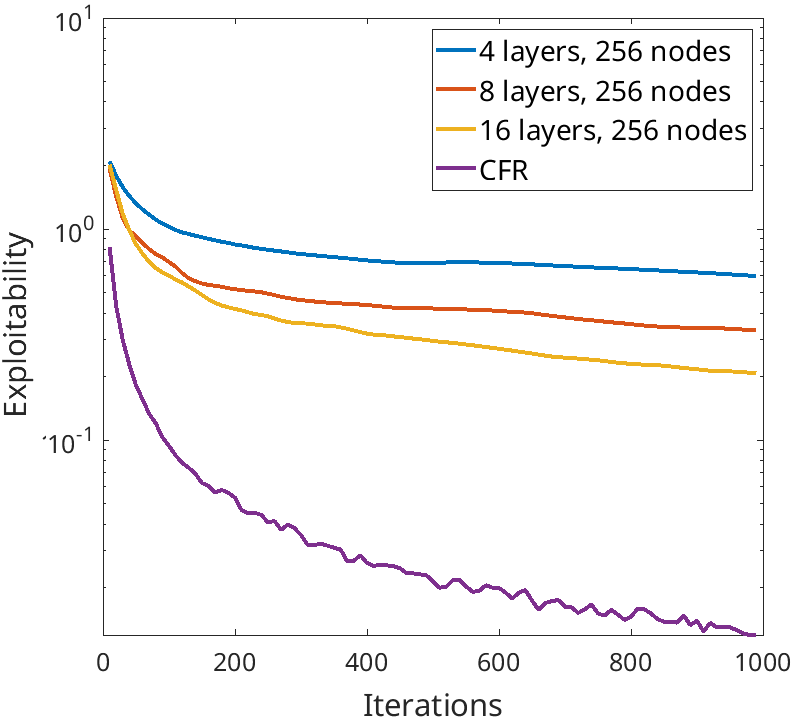
\includegraphics[scale=0.26]{Figures/rcfr_leduc_parameters2.png}
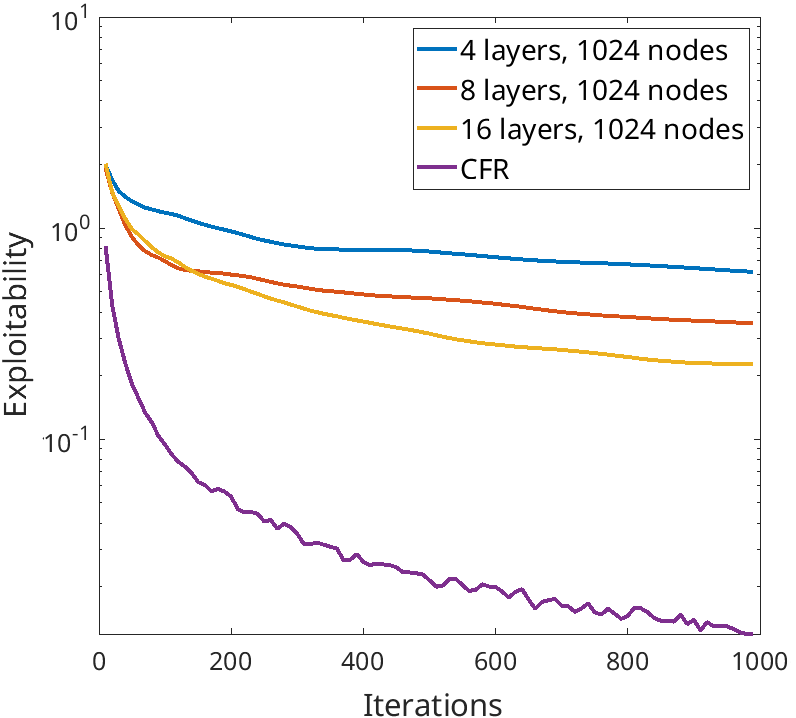
\includegraphics[scale=0.26]{Figures/rcfr_leduc_parameters3.png}
\caption{Influence of network parameters on CFR and RCFR exploitability}
\label{fig:rcfr_kuhn}
\end{figure}
\FloatBarrier 

Again, we examine the exploitability of CFR and RCFR in an experiment of 1000 iterations. CFR still outperforms RCFR in all cases. It is, however, remarkable how increasing the number of layers causes a monotone decrease in exploitability, which was not the case when learning Kuhn Poker. Still, increasing the number of nodes per layer has no clear influence on exploitability.

Table \ref{tbl:leduc_times} shows how long one iterations takes to compute. Again, using RCFR is slower than using CFR, as expected. It should be noted that the difference in execution time between CFR and RCFR is much smaller for Leduc Poker than for Kuhn Poker: in Kuhn Poker, introducing regression multiplied the time for one iteration by at least 30. In Leduc Poker, this factor is only 3.

\FloatBarrier
\begin{table}
	\centering
	\begin{tabular}{|l|r|}
	\hline
	Algorithm & Average time per iteration (milliseconds)\\
	\thickhline
	CFR & 946 \\
	\thickhline
	RCFR, 4 layers, 64 nodes& 2700 \\
	\hline
	RCFR, 4 layers, 256 nodes & 2539 \\
	\hline
	RCFR, 4 layers, 1024 nodes & 2569 \\
	\thickhline
	RCFR, 8 layers, 64 nodes & 3164 \\
	\hline
	RCFR, 8 layers, 256 nodes  & 3289 \\
	\hline
	RCFR, 8 layers, 1024 nodes  & 3717 \\
	\thickhline
	RCFR, 16 layers, 64 nodes & 4549 \\
	\hline
	RCFR, 16 layers, 256 nodes & 4725 \\
	\hline
	RCFR, 16 layers, 1024 nodes & 4364 \\
	\hline
	\end{tabular}
	\caption{Computation time of one iteration for Leduc Poker, averaged over 50 episodes}
	\label{tbl:leduc_times}
\end{table}
\FloatBarrier

These results confirm some of our expectations with regards to RCFR:
\begin{itemize}
\item{RCFR is no viable alternative for CFR when the number of information states is small enough to execute CFR: the error introduced by regression makes it much harder to reach an equilibrium. Both Kuhn Poker and Leduc Poker are games of manageable size, so using RCFR is not recommended (even with a neural network as regressor).}
\item{The computation time for one iteration of RCFR is much longer than the time for one iteration of CFR. Therefore, to save time, it is not recommended to use RCFR when this is not necessary.}
\item{For larger games, using an expressive regressor (such as a multi-layered neural network) improves the effectivity of RCFR (at the cost of increased computation times).}
\end{itemize}



\bibliographystyle{plainnat}
\bibliography{lit}
\section*{Appendix}
\subsection{Time spent}
\end{document}

CFR
Regression CFR
CFR-BR
Deep CFR